\documentclass{article}
\usepackage{subcaption}
\usepackage{amsmath}
\usepackage{mathtools}
\usepackage{hyperref}
\usepackage{polski}
\usepackage[utf8]{inputenc}
\usepackage{titlesec}
\usepackage{scalerel}
\usepackage{upquote}
\usepackage{multicol}
\usepackage{graphicx}
\usepackage{tabularx}
\usepackage{blindtext}
\usepackage{color}
\usepackage{colortbl}
\usepackage{amsmath}
\usepackage{algorithm}
\usepackage[noend]{algpseudocode}
\usepackage{multicol}
\usepackage{braket}
\usepackage[dvipdfmx]{media9}
\definecolor{dkgreen}{rgb}{0,0.6,0}
\definecolor{gray}{rgb}{0.5,0.5,0.5}
\definecolor{mauve}{rgb}{0.58,0,0.82}
\usepackage{geometry}
 \geometry{
 a4paper,
 total={170mm,257mm},
 left=20mm,
 top=20mm,
 }
\usepackage{placeins}
\usepackage{svg}
\newcolumntype{s}{>{\columncolor{yellow}}c}
\newcolumntype{h}{>{\columncolor{pink}}c}
\usepackage{listings}
\usepackage{float}

\lstset{frame=tb,
  language=Matlab,
  aboveskip=3mm,
  belowskip=3mm,
  showstringspaces=false,
  columns=flexible,
  basicstyle={\small\ttfamily},
  numbers=none,
  numberstyle=\tiny\color{gray},
  keywordstyle=\color{blue},
  commentstyle=\color{dkgreen},
  stringstyle=\color{mauve},
  breaklines=true,
  breakatwhitespace=true,
  tabsize=3
}
\usepackage[utf8]{inputenc}
\titleclass{\subsubsubsection}{straight}[\subsection]

\newcounter{subsubsubsection}[subsubsection]
\renewcommand\thesubsubsubsection{\thesubsubsection.\arabic{subsubsubsection}}

\titleformat{\subsubsubsection}
  {\normalfont\normalsize\bfseries}{\thesubsubsubsection}{1em}{}
\titlespacing*{\subsubsubsection}
{0pt}{3.25ex plus 1ex minus .2ex}{1.5ex plus .2ex}
\makeatletter
\def\toclevel@subsubsubsection{4}
\def\l@subsubsubsection{\@dottedtocline{4}{7em}{4em}}
\makeatother
\setcounter{secnumdepth}{4}
\setcounter{tocdepth}{4}


\title{Podstawy Obliczeń Komputerowych\\ Laboratorium 2}
\author{Kamil Czop 259613 \\ Łukasz Majchrzak 262761 \\ Wtorek 11:15TN - Y02-37c - Dr inż. Konrad Kluwak}
\date{16 czerwca 2023}

\begin{document}

\maketitle
\section{Metody interpolacji wielomianowej}
\subsection{Cel ćwiczeń}
Celem wykonanego laboratorium było wykorzystanie dowolnego algorytmu interpolacji wielomianowej oraz interpolacji wykorzystującej funkcje sklejające.
\subsection{Dane}
\begin{center}
    
    \begin{tabular}{|h|c|c|c|c|c|}
        \hline
        $x$ & $10$ & $20$ & $30$ & $40$ & $50$ \\
        \hline
        $y = cos(x)$ & $0.98$ & $0.93$ & $0.86$ & $0.76$ & $0.64$ \\
        \hline
    \end{tabular}\\
Szukane $x$: $21^{\circ}$
\end{center}
\section{Metoda Lagrange}
Wielomianowa metoda interpolacyjna wykorzystuje zależność:
$$W(x) = \sum^n_{i=0}y_i=\frac{\varphi_i(x)}{\varphi_i(x_i)} = \sum^n_{i=0}\frac{\prod j \neq i (x - x_j)}{j \neq i (x_i - x_j)}$$
\begin{figure}[H]
    \begin{multicols}{2}
        \null \vfill
        \begin{algorithm}[H]
        \caption{Wstępny algorytm lagrange}\label{euclid}
        \begin{algorithmic}[1]
        \Require{$x_{1} \dots x_{N}, y_{1} \dots y_{N}, x_s$}
        \Ensure{$y_s$}
            \Procedure{Lagrange-old}{}
                \State{$res \gets 0$}
                \For {$i \gets 1$ to $N$}
                    \State{$a \gets y(i)$}
                    \State{$a_d \gets 1$}
                    \State{$res_{seg} = 1$}
                    \For{$j \gets 1$ to $n$}
                        \If {$j \neq i$}
                            \State {$a_d \gets a_d * (x_i - x_j)$}
                            \State {$res_{seg} \gets res_{seg} * (x_s - x_j$}
                        \EndIf
                        \State \textbf{Next} $j$
                    \EndFor
                    \State{$a \gets a / a_d$}
                    \State{$res_{seg} = res_{seg}*a$}
                    \State{$res = res + res_{seg}$}
                    \State \textbf{Next} $i$
                \EndFor
                \State \textbf{Stop}
            \EndProcedure
        \end{algorithmic}
\end{algorithm}
        \vfill \null
        \par
        \begin{figure}[H]
            \centering
            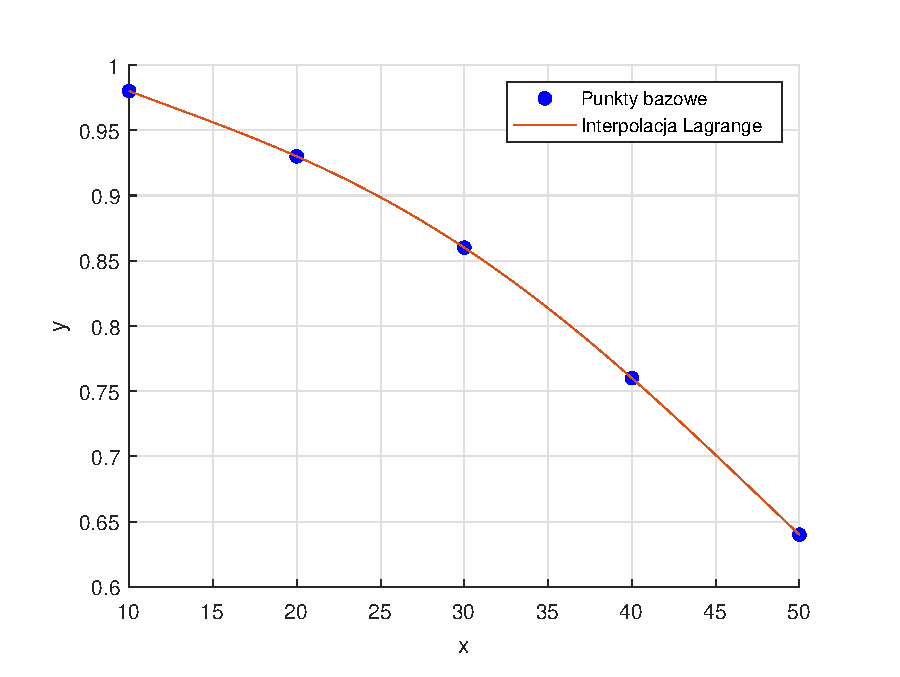
\includegraphics[width=\linewidth]{newImg/lagrange.eps}
        \caption{Interpolacja metodą Lagrange'a}
            \label{fig:my_label}
        \end{figure}
Dla $x = 21$ wartość interpolowana wynosi: 0.9242.
    \end{multicols}
\end{figure}
        Wykorzystywany w pierwsej wersji algorytm nie jest optymalny, ani natywny względem metod dostępnych w środowisku MATLAB. Zaprezentowany pseudokod korzysta z własności iteracyjnych algorytmu sumując kolejno wyznaczone elementy wielomianu.\\ Krzywa uzyskana jako całościowy wynik interpolacji przechodzi przez wszystkie punkty, co sugeruje prawidłowość działania implementacji metody.
\section{Metoda sześciennych funkcji sklejanych - Cubic Spline}
Metoda funkcji sklejanych wskazuje nazwą iż do interpolacji wykorzystujemy więcej niż jedną funkcję. Cubic Spline partycjonuje oś x celem utworzenia sześciennych funkcji których krzywe łączą się w jedno w znanych nam punktach badanej funkcji bazowej.
 \begin{figure}[H]
            \centering
            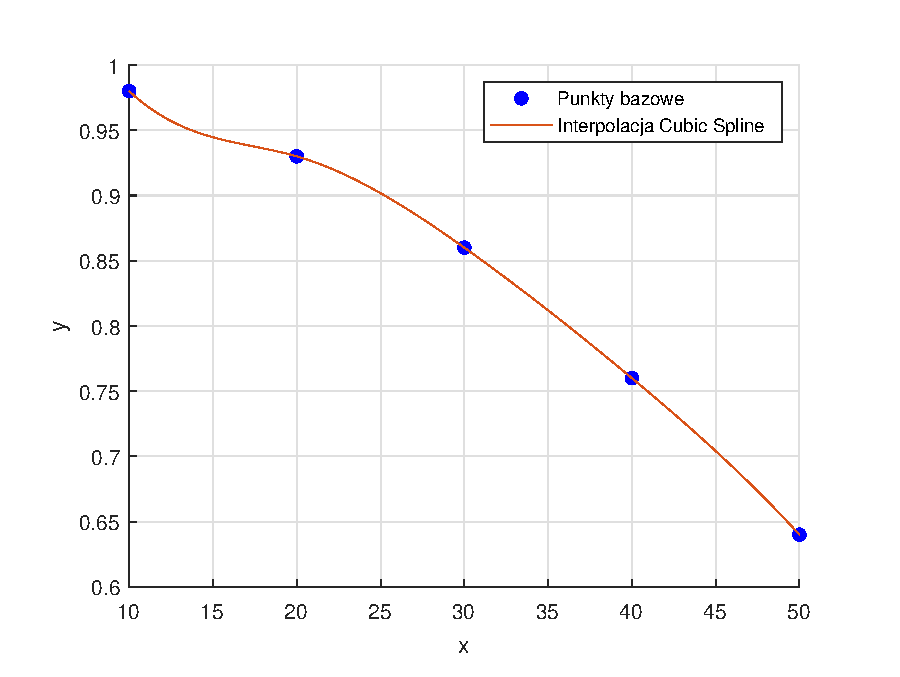
\includegraphics[width=\linewidth]{newImg/CubicSpline.eps}
        \caption{Interpolacja wykorzystująca Cubic Spline}
            \label{fig:my_label}
        \end{figure}
Uzyskano wartość dla szukanego x : $y \approx 0.9259$
 \begin{figure}[H]
            \centering
            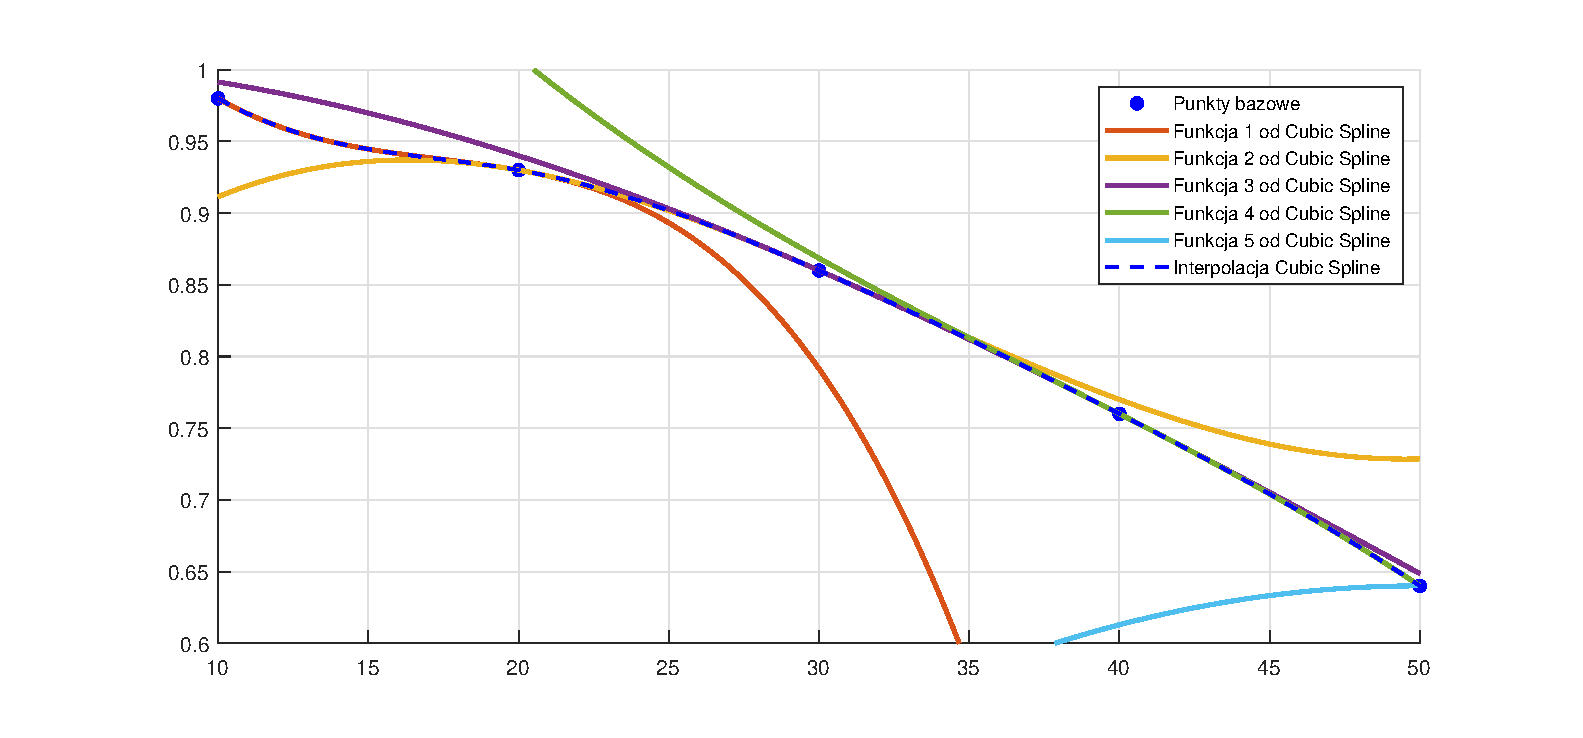
\includegraphics[width=\linewidth]{newImg/CSfunc.eps}
        \caption{Poszczególne "podfunkcje" sklejające}
            \label{fig:my_label}
        \end{figure}
Na załączonym wykresie dokładnie widać "sklejanie funkcji", gdzie pierwsza funkcja odwzorowywuje $x\in[10:20)$, druga funkcja $x\in[20:30)$, trzecia $x\in[30:40)$, czwarta $x\in[40:50)$ oraz piąta nie wykorzystana w zakreślonym obszarze $x\in[50:\infty)$.
\begin{figure}[H]
    \begin{multicols}{2}
        \begin{figure}[H]
            \centering
            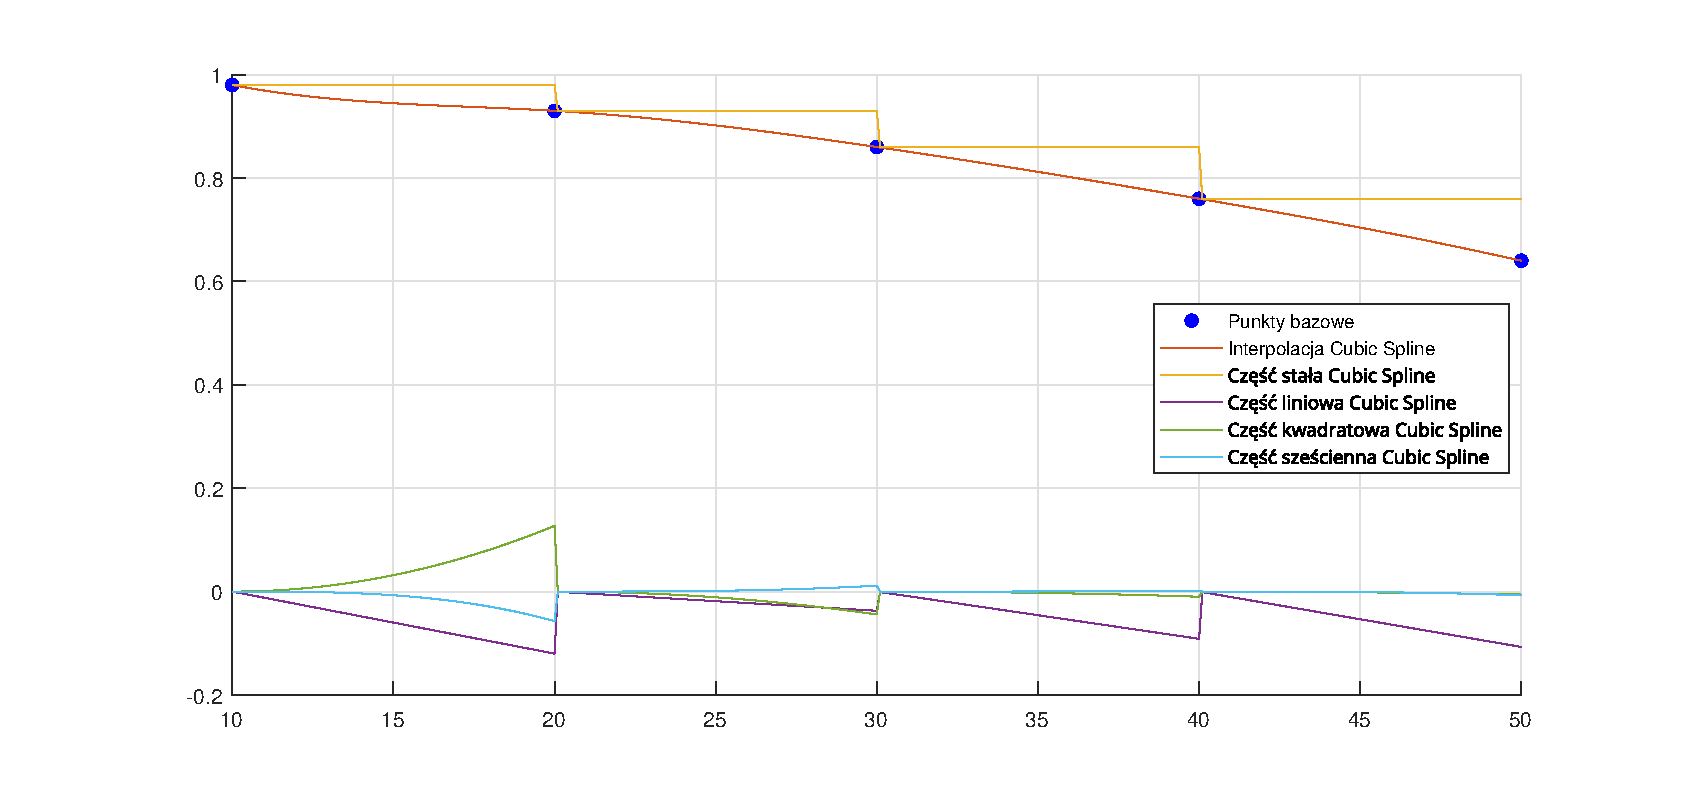
\includegraphics[width=\linewidth, trim={2cm 0cm 1.4cm 0cm}]{newImg/CSsegments.eps}
        \caption{Poszczególne wartości poziomów wartości w wielomianie}
            \label{fig:my_label}
        \end{figure}
        \par
        \null \vfill
        Na załączonym wykresie można zauważyć jak utworzone funkcje się zmieniają, w szczególności jak przejżymy przebieg stałej części parametru $a$, gdzie widać "schodkowanie", wraz ze przejściem do wartości punktu bazowego.\\
        W interpolowanym przypadku, część liniowa o parametrze $b$ była zawsze ujemna, wartość $b$ była wystarczająco wysoka by ukazać kształt piłokształtny na wykresie.
        \vfill \null
    \end{multicols}
\end{figure}
Wartości parametrów
\begin{center}
    \begin{tabular}{|h|c|c|c|c|c|}
        \hline
        $a$ & $0.9800$ & $0.9300$ & $0.8600$ & $0.7600$ & $0.6400$ \\
        \hline
        $b$ & $-0.0120$ & $-0.0037$ & $-0.0091$ & $-0.0107$ & $0$\\
        \hline
        $c$ & $0.0013$ & $-4.46e-4$ & $-0.0001$ & $-5.71e-5$ & $-2.71e-5$ \\
        \hline
        $d$ & $-5.71e-5$ & $1.14e-5$ & $1.42e-6$ & $-7.14e-6$ & $0$\\
        \hline
    \end{tabular}
\end{center}
\subsection{Porównanie}
\begin{figure}[H]
    \centering
    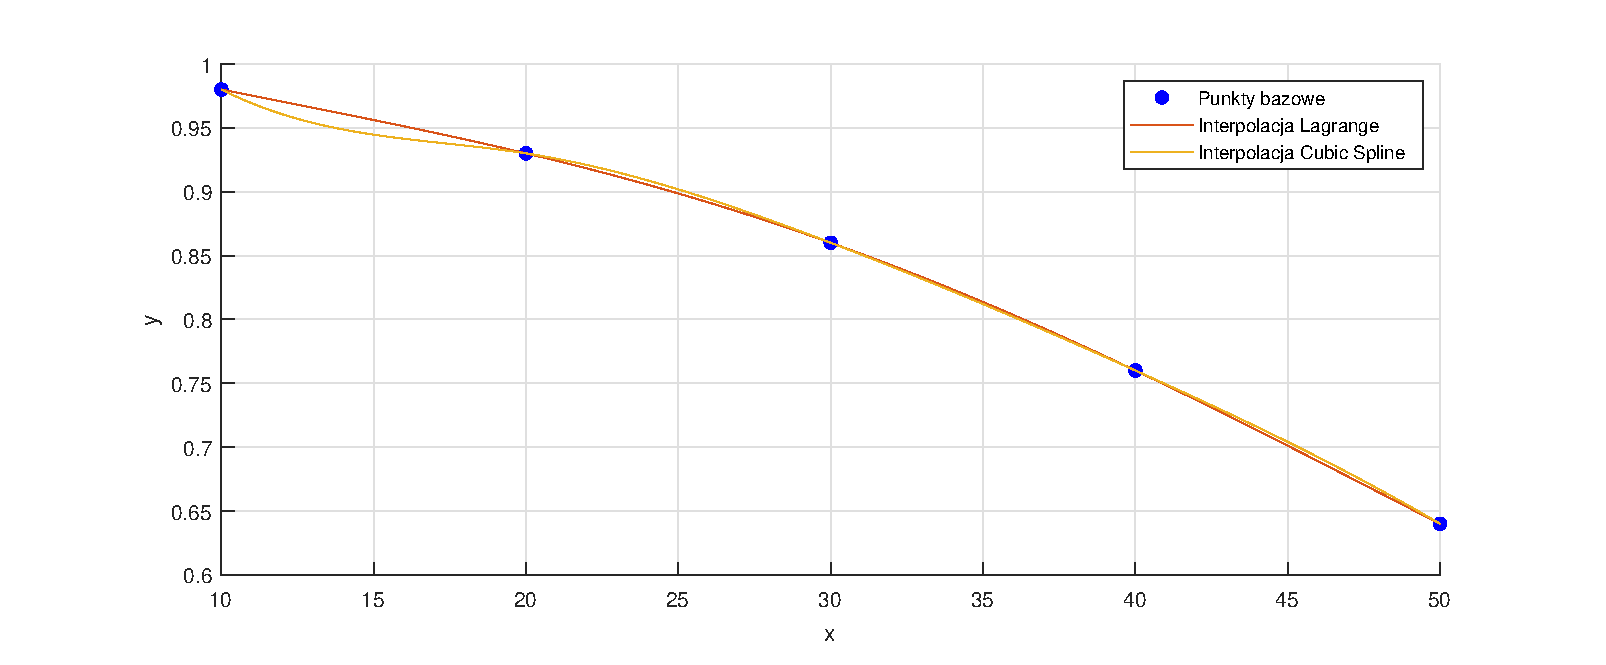
\includegraphics{newImg/compCSLg.eps}
    \caption{Porównanie interpolacji Cubic Spline i metody Lagrange'a}
    \label{fig:enter-label}
\end{figure}
\section{Wektory własne i wartości własne macierzy}
\subsection{Dane}
$$A = \begin{bmatrix}
    3 & 1 & 2 \\
    1 & 8 & 1 \\
    2 & 1 & 1
\end{bmatrix}$$
\subsection{Uzyskany wynik}
\begin{itemize}
    \begin{multicols}{2}
    \item Wartość własna: $8.0393$ 
    \par
    \item Wektor własny: $\begin{bmatrix} 0.2447 \\ 0.9502 \\ 0.1930\end{bmatrix}$
    \end{multicols}
\end{itemize}
\section{Github, bibliografia, dokumentacja}
\begin{itemize}
    \item \url{https://github.com/Myknakryu/pok-2023}
    \item \url{https://traf-barak.pwr.edu.pl/wp-content/uploads/2020/08/Raport.pdf}
    \item \url{https://www.youtube.com/watch?v=2YmCaxcKyBY}
\end{itemize}
\end{document}
